\documentclass[12pt,letterpaper,noanswers]{exam}
\usepackage[usenames,dvipsnames,svgnames,table]{xcolor}
\usepackage[margin=0.9in]{geometry}
\renewcommand{\familydefault}{\sfdefault}
\usepackage{multicol}
\pagestyle{head}
\header{AM 111 Class 20}{}{Initial value problems: differential equations, p.\thepage}
\runningheadrule
\headrule
\usepackage{siunitx}
\usepackage{graphicx} % more modern
\usepackage{amsmath} 
\usepackage{amssymb} 
\usepackage{hyperref}
\usepackage{tcolorbox}
\usepackage{enumitem}
\def\mbf{\mathbf}
\newcommand{\vc}[1]{\boldsymbol{#1}}
\def\dsst{\displaystyle}
\DeclareMathOperator*{\argmin}{arg\,min} % thin space, limits underneath in displays
\usepackage{listings}

\begin{document}
 \pdfpageheight 11in 
  \pdfpagewidth 8.5in

\noindent 

\section*{Preliminaries}

\begin{itemize}
\itemsep0pt
\item Your problem set and project log are due tomorrow.
\item There is a skill check in the next class.
\end{itemize}


\noindent\textbf{Big picture}

Today: For methods of approximating solutions to ODEs, how do we find the local truncation error?  How can we adjust the step size of the method to reduce the number of steps while meeting desired error tolerances?

\vspace{0.2cm}
\hrule
\vspace{0.2cm}

\noindent \textbf{Skill check practice}
 The midpoint method is given by $y_{k+1} = y_k + h\psi(t_k,y_k,h)$ where $\psi(t_k,y_k,h) = f(t_k+h/2,y_k+hf(t_k,y_k)/2)$.

Use Taylor expansion to first order to write $f(t_k+h/2,y_k+hf(t_k,y_k)/2)$ in terms of $f(t_k, y_k)$,$\dfrac{\partial f}{\partial t}(t_k,y_k)$, $\dfrac{\partial f}{\partial y}(t_k,y_k)$, and $\mathcal{O}(h^2)$.

\emph{You'll be asked to use Taylor expansion to first order to rewrite a method in this way.}


\vspace{0.2cm}
\hrule
\vspace{0.2cm}

\noindent \textbf{Skill check solution}

Answer: $f(t_k+h/2,y_k+hf(t_k,y_k)/2) = f(t_k,y_k) + \dfrac{h}{2} \dfrac{\partial f}{\partial t}(t_k,y_k) + \dfrac{h}{2}f(t_k,y_k) \dfrac{\partial f}{\partial y}(t_k,y_k) + \mathcal{O}(h^2)$


More explanation:

Taylor expanding about $f(t_k, y_k)$, the displacement in time is $\Delta t = h/2$ and the displacement in $y$ is $\Delta y = hf(t_k,y_k)/2$.

In general, $f(t+\Delta t, y+\Delta y) = f(t,y) + \Delta t \dfrac{\partial f}{\partial t}(t,y) +  \Delta y \dfrac{\partial f}{\partial y}(t,y) + \text{higher order terms}$





\vspace{0.2cm}
\hrule
\vspace{0.2cm}


\section*{Ordinary differential equations}
\subsection*{Explicit methods}
 (see Greenbaum and Chartier \S 11.2 and Sauer \S 6)

% \begin{tcolorbox}
% Let $w_k$ denote the approximation to $y(t_k)$ produced by our numerical method.

% An \textbf{explicit} one-step method can be written in the form $w_{k+1} = w_k + h \psi(t_k,w_k,h)$ where $\psi(t_k,w_k,h)$ is an estimate of the effective slope of $y(t)$ over the interval $[t_k,t_{k+1}]$.

% \emph{Note: I gave a definition for \textbf{one step} last class that was incorrect: it was actually the definition for \textbf{one stage}}
% \end{tcolorbox}


 

\begin{enumerate}
    \item For the following three methods, provide a formula for $\psi(t_k,w_k,h)$, the estimated slope used over the interval $[t_k,t_{k+1}]$
    \begin{enumerate}
    \item Euler: $w_{k+1} = w_k + hf(t_k,w_k)$.
    \vspace{1cm}
    \item midpoint method: $w_{k+1} = w_k + h\psi(t_k,w_k,h)$ where the slope is given by using a half step of Euler's method to find an estimate of the midpoint of the interval, and the slope at the midpoint is used for the whole interval
    \vspace{1.5in}
    \item explicit trapezoid:
    
    $s_1 = f(t_k,w_k)$, 
    
    $s_2 = f(t_k + h, w_k + hs_1)$
    
    $w_{k+1} = w_k + \frac{h}{2}(s_1 + s_2)$
    \vspace{1in}
    \end{enumerate}
\end{enumerate}

% \begin{tcolorbox}
% If local truncation error is given by $e_k \leq Ch^{n+1}$ then global truncation error is $\mathcal{O}(h^n)$ and the method is said to be order $n$.  For details see Sauer \S 6.1.2 and \S 6.2.1.

% \emph{Think of global truncation error as being approximately the sum of the local errors.}
% \end{tcolorbox}

% We'll need Taylor's theorem in two dimensions (because $f(t,y)$) to identify the location truncation error.

% \begin{tcolorbox}
% Taylor's theorem in two dimensions:

% Let $S = (a,b)\times(c,d)$ be a set in $(t,y)$.  Let $(t_0,y_0)\in S$ and $(t_0+h,y_0+k)\in S$ be given points and assume $f(t,y)$ is $n+1$ times continuously differentiable for all $(t,y) \in S$.  Then

% \begin{align*}f(t_0+h,y_0+k) =& f(t_0,y_0) + hf_t(t_0,y_0) + kf_y(t_0,y_0) \\
% &+ \frac{h^2}{2}f_{tt}(t_0,y_0) + hkf_{ty}(t_0,y_0) + \frac{k^2}{2}f_{yy}(t_0,y_0) + ... \\
% = & f(t_0,y_0) + \sum\limits_{j=1}^n \frac{1}{j!}\left[h\frac{\partial}{\partial t} + k\frac{\partial}{\partial y} \right]^j \left.f(t,y)\right\vert_{(t,y) = (t_0,y_0)} \\
% &+  \frac{1}{(n+1)!} \left[h\frac{\partial}{\partial t} + k\frac{\partial}{\partial y} \right]^{n+1}\left.f(t,y)\right\vert_{(t,y) = (c_1,c_2)}
% \end{align*}
% for $t_0 \leq c_1 \leq t_0 +h,y_0\leq c_2\leq y_0+k$
% \end{tcolorbox}



\begin{enumerate}[resume]
    \item (explicit trapezoid)
The explicit trapezoid method is
$w_{k+1} = w_k + \frac{h}{2}\left(f(t_k,w_k) + f(t_k+h, w_k + hf(t_k,w_k))\right)$

\emph{This is a two stage method.  This method is called improved Euler, trapezoid method, or Heun method.}
    \begin{parts}
    \item To identify the local truncation error, start by Taylor expanding $f(t_k + h, w_k+hf(t_k,w_k)$ about $(t_k, w_k)$.  It is sufficient to expand to first order (following the format below).
    
    \emph{To do a 2D Taylor expansion to first order, $f(t+h, y + \Delta) \approx f(t,y) + h\dfrac{\partial f}{\partial t}(t,y) + \Delta \dfrac{\partial f}{\partial y}(t,y) + \mathcal{O}(h^2)$ (for the dropped terms to be $\mathcal{O}(h^2)$, I am assuming that $\Delta$ is $\mathcal{O}(h)$).}
    \vspace{2in}
    
    \item The local truncation error is $\vert y_{k+1} - w_{k+1}\vert$ (after assuming that $w_k = y_k$).  Do this subtraction to show that it is $\mathcal{O}(h^3)$.
    \vspace{1in}
    \end{parts}

    

     \item (midpoint)
The midpoint method is
$w_{k+1} = w_k + \frac{h}{2}\left(f(t_k,w_k) + f(t_k+h, w_k + hf(t_k,w_k))\right)$.  Use Taylor expansion to find the local truncation error.
\vspace{1.5in}

    
    \item The global error for explicit trapezoid will be $\mathcal{O}(h^2)$ so it is said to be a second order method (while Euler is a first order method).  How can you tell the order of the methods in the plot of error below?  What happens to the error from explicit trapezoid as step size becomes small (and why)?

\emph{Note: these calculations are more time-intensive to run, which is why $h$ stops at $10^{-8}$.}
\end{enumerate}


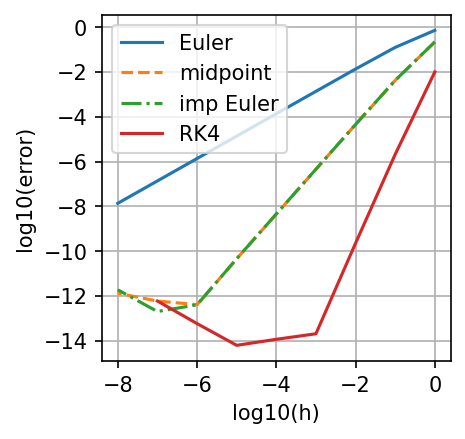
\includegraphics[]{img/C18error.png}
\subsection*{Systems of first order equations}
% \begin{tcolorbox}
% The two methods we have encountered so far work for initial value problems, which involve first order differential equations.

% A second order differential equation can be turned into a \textbf{system} of two first order differential equations (and an $n$th order differential equation into  a system of $n$ first order equations).
% \end{tcolorbox}
\begin{enumerate}[resume]
\item Convert the second-order differential equation $y'' = a(y')^2 +yy' - \cos t$ to a system of two first order equations.
\begin{parts}
\item Set $y_1 = y$ and define the new variable $y_2 = y'$.  Rewrite the equation above, by replacing $y''$ with $y_2'$.  Replace $y'$ with $y_2$.  Replace $y$ with $y_1$.
\vspace{1cm}
\item Write down your system.  $y_1' = y_2$ is the first equation in the system.  $y_2' = ??$ is the second equation.
\vspace{1.5cm}
\end{parts}
\item Apply one step of Euler's method to initial value problem \[\left\{\begin{array}{l}
y_1' = y_2 - y_1^2 \\
y_2' = y_1 -ty_2^3 \\
y_1(1) = 0 \\
y_2(1) = 3 \end{array}\right.\]
$\begin{array}{l}
w_{0,1} = 0\\
w_{0,2} = 3
\end{array}$. Set up expressions for $\begin{array}{l}
w_{1,1}\\
w_{1,2}
\end{array}$
\vspace{1in}
\end{enumerate}




% \begin{tcolorbox}
% Explicit \textbf{Runge-Kutta} methods use intermediate estimates of $y$ in the interval $[t_k,t_{k+1}]$ in order to create $\psi(t_k,w_k,h)$.  
% \begin{itemize}
% \itemsep0pt
%     \item Explicit trapezoid is a Runge-Kutta method.  So is the midpoint method.  Recall that their global truncation error is 2nd order, so it is called second order Runge-Kutta methods.
%     \item The \textbf{classical fourth-order Runge-Kutta method} (RK4) is given by 
    
%     $s_1 = f(t_k,w_k)$, 
    
%     $s_2 = f(t_k+h/2,w_k+\frac{h}{2}s_1)$
    
%     $s_3 = f(t_k + h/2,w_k + \frac{h}{2}s_2)$
    
%     $s_4 = f(t_k+h, h_k + hs_3)$
    
%     $\psi(t_k,w_k,h) = \frac{1}{6}(s_1+2s_2+2s_3+s_4)$
% \end{itemize}

% We will not Taylor expand to show this has local truncation error of 5th order.
% \end{tcolorbox}
\begin{enumerate}[resume]
\item Let $\frac{dy}{dt} = ty$, $y(0) = 1$.  Write Python code to implement forward Euler to estimate $y(1)$ using steps of size $0.1$.
\vspace{1in}

\item Modify your code to use RK4.
\vspace{1in}

\item How would your code need to change to solve a system, $\frac{dy_1}{dt} = t(y_1+y_2)$, $\frac{dy_2}{dt} = \sin y_2$, $y_1(0) = 1, y_2(0) = 1$?
\end{enumerate}

\subsection*{Variable step size methods}

% Main idea: approximate the error on the current step, $e_k$.  If $e_k$ (absolute) and/or $e_k/\vert w_k\vert$ (relative) error is below tolerance, keep the step.  Otherwise, lower the step size.  If error is far below tolerance, increase the step size for the next step.

% Goal: use large step sizes while meeting error tolerances.

% How is the error estimated?

% In our integration methods, we used the same method with two different step sizes to approximate error.  For this problem, we use methods with two different orders: and RK 23 pair, or an RK 45 pair.

\begin{enumerate}[resume]
\item Combine explicit trapezoid (order 2) with a rule similar to Simpson's (order 3).

Let

$s_1 = f(t_k,w_k)$

$s_2 = f(t_k + h, w_k + hs_1)$

$s_3 = f\left(t_k+ h/2, w_k + h/2\frac{s_1+s_2}{2}\right)$

$w_{k+1} = w_k + h\frac{s_1+s_2}{2}$

$z_{k+1} = w_k + h\frac{s_1+4s_3+s_2}{6}$.

\begin{enumerate}
\item How many additional function evaluations (evaluations of $f$) were used to create $w_{k+1}, z_{k+1}$ compared to just creating $w_{k+1}$?

\item How can you use $w_{k+1}$ and $z_{k+1}$ to approximate the error?

\item Does it make more sense to use $w_{k+1}$ or $z_{k+1}$ as the starting value for the next step?
\end{enumerate}
\item Matlab's \texttt{ode23} (Bogacki-Shampine order 2/order 3 embedded pair)

$s_1 = f(t_k,w_k)$

$s_2 = f(t_k + \frac{h}{2}, w_k + \frac{h}{2}s_1)$

$s_3 = f(t_k + \frac{3h}{4}, w_k + \frac{3h}{4}s_2)$

$z_{k+1} = w_k + h\frac{2s_1+3s_2+4s_3}{9}$.

$s_4 = f(t_k+ h, z_{k+1})$

$w_{k+1} = w_k + h\frac{7s_1+6s_2+8s_3+3s_4}{24}$

$z_{k+1}$ is order 3 and $w_{k+1}$ is order 2.

Compare $s_1$ and $s_4$.  This method design is called `first same as last' (FSAL).  What is that referring to?

\end{enumerate}

\end{document}